\cotefile{73}
\scanpage{18}
\mspage{4}

% top centre
\unsure{quadrilatère}

% upper left
\figure{\begin{tikzpicture}[x=.83cm,y=.83cm,>=stealth]
\draw[->] (-2.6,-.06)--(3.25,.14);
\draw[->] (-.87,-2.02)--(.78,2.32);
\fill (-1.38,-.01) circle (1.6pt) node[below=2pt] {$s_0$};
\draw (.01,.01) ++(1.72,.045) circle (1.6pt) node[below=2pt] {$s_2$};
\fill (-.46,-.93) circle (1.45pt) node[right] {$s_1$};
\fill (.47,1.52) circle (1.45pt) node[right] {$s_3$};
\end{tikzpicture}}

% upper half, coordinate rows 1–4
\[
\begin{aligned}
(\unsure{a|\alpha}-1,\deleted{\unsure{a+1|a+}}0)&\qquad (-(a-1),b-1)=(-a+1,b-1) &&u_0\\
(0,b-1)&\qquad (a+1,-(b-1))=(a+1,-b+1) &&u_1\\
(a+1,0)&\qquad (-(a+1),b+1)=(-a-1,b+1) &&u_2\\
(0,b+1)&\qquad (a-1,-(b+1))=(a-1,-b-1) &&u_3
\end{aligned}
\]

% middle, product rows 1–4
\[
\begin{aligned}
(1-a)(1-b)+(1-b)(a+1)&=2(1-b)=f_{\unsure{1}}\\
(a+1)(b+1)+(a+1)(\deleted{\unsure{b}}1-b)&=2(a+1)=f_2\\
(a+1)(b+1)+(b+1)(1-a)&=2(b+1)=f_3\\
(a-1)(b-1)\deleted{\unsure{+}}\unsure{-}(b+1)(a-1)&=2(1-a)=f_0
\end{aligned}
\]

% below products, two columns
\[
f_1+f_3=f_2+f_0=\deleted{4}\unsure{v|\nu}
\quad\Big/\quad
\begin{aligned}
 f_3-f_1&=\text{\textcircled{$b$}}v\\
 f_2-f_0&=\text{\textcircled{$a$}}v
\end{aligned}
\]

% lower left, beside wedge identity
\figure{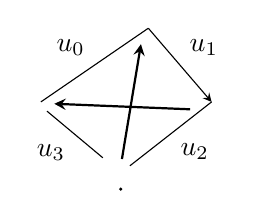
\begin{tikzpicture}[scale=.78,>=stealth]
\draw (-1.4,0)--(.35,1.2) node[midway,above left] {$u_0$};
\draw[->] (.35,1.2)--(1.38,0) node[midway,above right] {$u_1$};
\draw (1.38,0)--(.05,-1.04) node[midway,below right] {$u_2$};
\draw (-.39,-.91)--(-1.30,-.15) node[midway,below left] {$u_3$};
\draw[->,thick] (1.03,-.12)--(-1.18,-.03);
\draw[->,thick] (-.08,-.93)--(.23,.94);
\fill (-.1,-1.42) circle (.8pt);
\end{tikzpicture}}

% lower third, beside and below quadrilateral
\[
\begin{aligned}
u_0\wedge u_1+u_2\wedge u_3&=u_1\wedge u_2+u_3\wedge u_0
 \overset{?}{=}\underbrace{(u_0+u_1)(u_1+u_2)}_{\begin{gathered}u_0\wedge u_1+u_0\wedge u_2\\{}+u_1\wedge u_2\end{gathered}}\\
u_3&=-(u_0+u_1+u_2)
\end{aligned}
\]

% lower third, line with cross-outs and pairing strokes
\[
\underbrace{u_0\wedge u_1}\deleted{\unsure{+}}\unsure{-|+}%
\underbrace{\underbrace{u_2\,(u_0}+u_1}+\deleted{u_2})
 =\underbrace{u_1\wedge u_2}+\underbrace{\underbrace{u_0\wedge(\deleted{u_0}+u_1}+u_2})
\]

% foot, right above long rule
\[
u_2\wedge\underbrace{(u_3+u_0+u_1)}_{-u_2}=0\qquad\text{\unsure{Ok|Oh}}
\]

% foot, left to right
\figure{\begin{tikzpicture}[x=.77cm,y=.72cm,>=stealth]
\draw (0,.2) .. controls (1,-.12) and (4.6,1.25) .. (6.6,.14) .. controls (8.5,-.7) and (10.6,-.53) .. (12,-.38);
\draw[->] (1.2,-.58)--(2.58,.53) node[midway,above left] {$u$};
\draw[->] (2.58,.53)--(3.17,-.53) node[midway,right] {$v$};
\end{tikzpicture}}

% foot left, below rule
\[
\deleted{u\wedge v=-(-v)\wedge(-u)}
\]

% foot centre
\figure{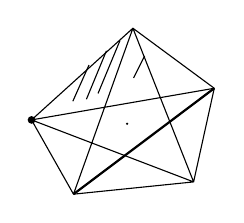
\begin{tikzpicture}[scale=.82]
\coordinate (a) at (-1.45,.08); \coordinate (b) at (.12,1.5);
\coordinate (c) at (1.38,.57); \coordinate (d) at (1.06,-.88); \coordinate (e) at (-.8,-1.07);
\draw (a)--(b)--(c)--(d)--(e)--cycle (a)--(c) (a)--(d) (b)--(d) (b)--(e) (e)--(c);
\draw[thick] (e)--(c); \fill (a) circle (1.7pt);
\draw (-.81,.37)--(-.56,.93) (-.60,.4)--(-.29,1.15) (-.42,.49)--(-.08,1.31) (.13,.73)--(.3,1.07);
\fill (.03,.02) circle (.55pt);
\end{tikzpicture}}

% archive sheet number: 24
